% Chapter 23 -- Claim: Language Models Can Read the News and Earn Returns
% Requires: amsmath, amssymb, booktabs, array, tabularx, graphicx, tcolorbox (breakable, skins), hyperref or url.
% Defines the callout box only if the preamble has not.
\providecolor{fenavy}{HTML}{1B2A6B}
\providecolor{feshade}{HTML}{F3F5FA}
\makeatletter
\@ifundefined{callout}{%
  \newtcolorbox{callout}{breakable, enhanced,
    colback=white, colframe=gray!70, boxrule=0.5pt, arc=1mm,
    borderline west={2.5pt}{0pt}{gray!70},
    left=8pt, right=8pt, top=4pt, bottom=4pt}%
}{}
\makeatother

\chapter{Claim: Language Models Can Read the News and Earn Returns}
\label{ch:23}

Markets run on words as much as numbers: earnings releases, analyst notes, central-bank statements and a constant stream of headlines. For most of the history of quantitative finance those words were invisible to models, which saw only prices and accounting figures. Text analysis changed that, first with word counts and dictionaries, then with machine-learned representations, and since 2023 with large language models that can read a headline and say whether it is good or bad news.

The early LLM results were remarkable. A 2023 study found that ChatGPT's reading of news headlines predicted next-day stock returns, and that a long--short strategy built on it earned a Sharpe ratio above 3 before costs. If a general-purpose model can read the news better than the market prices it, every investor with an API key has a new edge.

The claim faces two problems that earlier chapters have prepared us for. The first is look-ahead: a model trained on the internet may already know what happened after the headline. The second is competition: a signal anyone can compute cheaply should not last. This chapter tests both.

By the end of the chapter you will be able to:

\begin{itemize}
  \item turn text into numbers with word counts, dictionaries and net tone, and explain why finance needs its own dictionaries;
  \item explain embeddings, contextual language models, FinBERT and zero-shot use of large language models;
  \item measure the effect of news with abnormal and cumulative abnormal returns, counting only returns that could have been traded;
  \item explain look-ahead bias and the distraction effect in pretrained models, and how post-cutoff testing and anonymization address them;
  \item compute how trading costs erode a daily news strategy;
  \item state the three parts of the claim and judge the evidence for each.
\end{itemize}

\section{Foundations: text as data, language models and event studies}
\label{sec:23-foundations}

\textbf{Text as data.} To use text in a statistical model, each document must become numbers. Gentzkow, Kelly and Taddy (2019) describe three steps: represent the text numerically, map that representation to a quantity of interest such as sentiment, and use the quantity in a model of outcomes such as returns.

\textbf{Bag of words and dictionaries.} The simplest representation counts words, ignoring their order. A \textbf{dictionary} (or lexicon) is a list of words tied to a meaning, such as positive or negative. A document's \textbf{net tone} is
\begin{equation}
  \text{tone} = \frac{\text{positive words} - \text{negative words}}{\text{positive words} + \text{negative words}}
  \label{eq:23-tone}
\end{equation}
which ranges from $-1$ to $+1$. Dictionaries are transparent and cheap, but they ignore context: ``not profitable'' counts as positive, and words that are negative in everyday English may be neutral in finance.

\textbf{Domain matters.} Loughran and McDonald (2011) found that almost three-quarters of the words a widely used general dictionary classifies as negative are not negative in financial text. Words such as \emph{tax}, \emph{cost}, \emph{liability}, \emph{capital} and \emph{crude} are routine in a 10-K. They built finance-specific word lists, which are now standard.

\textbf{Embeddings and language models.} An \textbf{embedding} maps a word, sentence or document to a vector, so that texts with similar meanings lie close together. Transformer language models such as BERT produce \textbf{contextual} embeddings, in which the same word gets a different vector in different sentences. FinBERT is BERT fine-tuned to classify financial sentiment. \textbf{Large language models} (LLMs) such as GPT-4 or Claude go further: they can be asked in plain language whether a headline is good or bad news, with no task-specific training. That is called \textbf{zero-shot} use.

\textbf{Event studies.} The effect of news on prices is measured with an event study. The \textbf{abnormal return} is the stock's return minus a benchmark, here the market's return. The \textbf{cumulative abnormal return} (CAR) adds abnormal returns over a window of trading days. For a trading signal, only returns after the news could have been acted on count: a headline released after the close can first be traded at the next day's close (Figure~\ref{fig:23-timing}).

\begin{figure}[htbp]
\centering
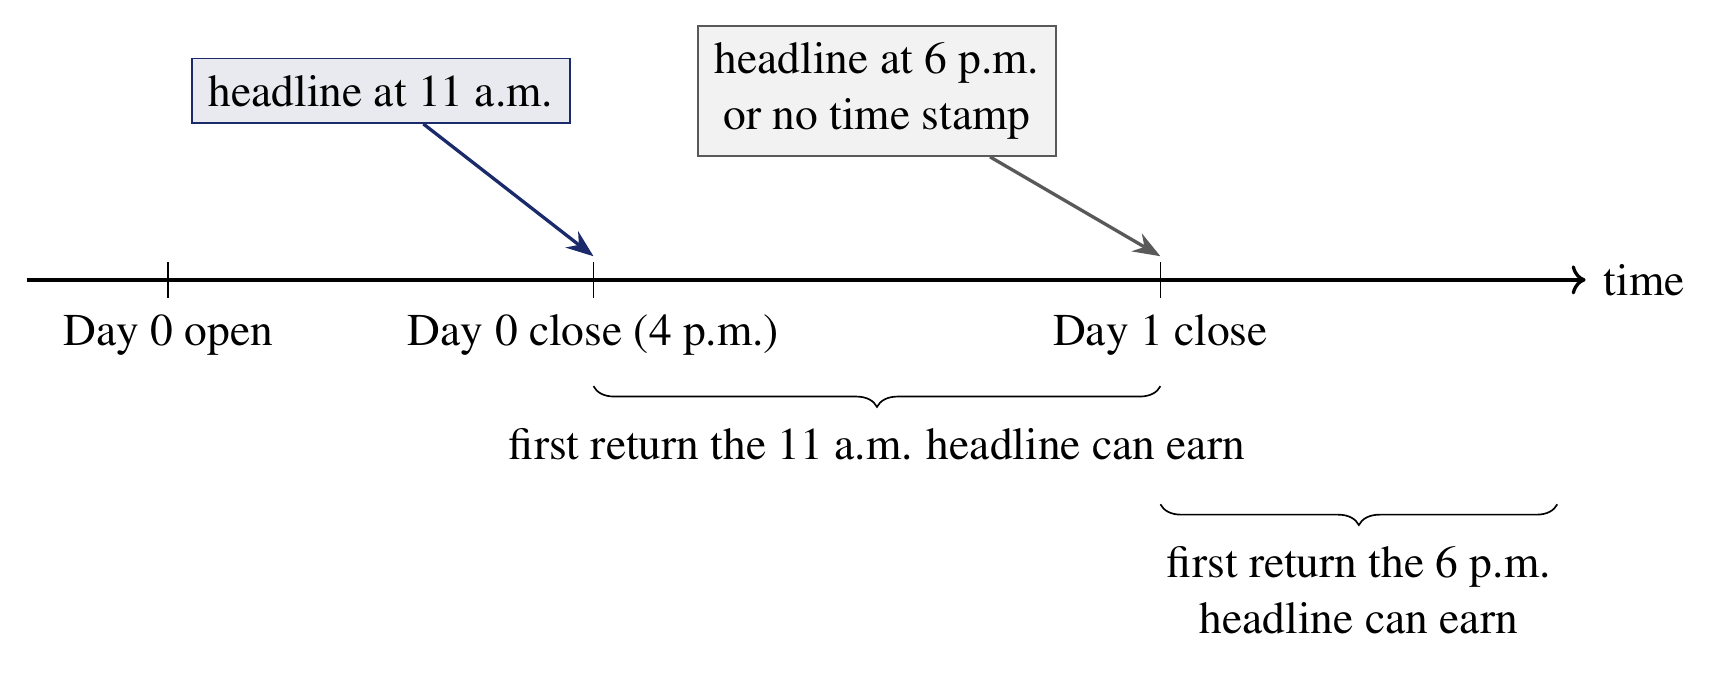
\includegraphics[width=0.9\linewidth]{images/fig23-1-timing.png}
\caption{When a headline can first be traded. News before the 4 p.m. close is traded at that day's close, so the first return it can earn is the next day's. News after the close, or without a time stamp, is traded at the next day's close. Returns on the day the news appeared are never counted.}
\label{fig:23-timing}
\end{figure}

\textbf{Look-ahead in pretrained models.} A language model's knowledge stops at its \textbf{training cutoff}. If a backtest uses headlines from before the cutoff, the model may have read later articles about the same events, and its ``forecast'' may reflect knowledge of the outcome. Glasserman and Lin (2023) also identified a \textbf{distraction effect}: a model's general knowledge of a well-known company can colour its reading of the headline. Removing company names (\textbf{anonymization}) and testing only on data after the cutoff address the two problems.

\textbf{Worked example.} A long--short strategy earns 20 basis points a day before costs, with a daily standard deviation of 1\% (Figure~\ref{fig:23-costs}).

\begin{itemize}
  \item Its annualized Sharpe ratio is $0.002/0.01 \times \sqrt{252} \approx 3.2$.
  \item If the whole book is replaced every day, the strategy completes one round trip on its long side and one on its short side each day. At 5 basis points per round trip, it pays 10 basis points a day in costs. Net return halves to 10 basis points and the Sharpe ratio falls to about 1.6.
  \item At 10 basis points per round trip, nothing is left.
\end{itemize}

\begin{figure}[htbp]
\centering
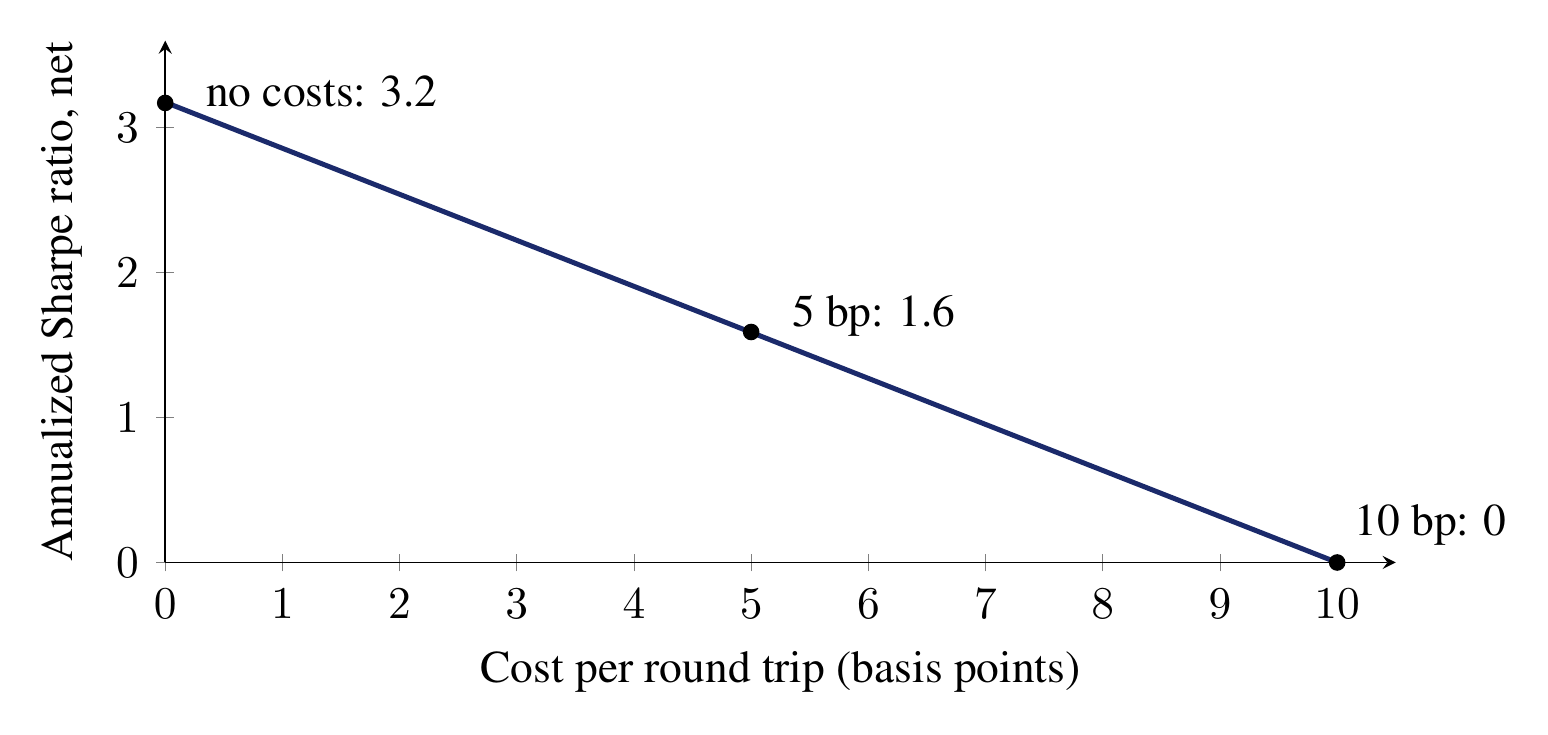
\includegraphics[width=0.85\linewidth]{images/fig23-2-cost-sharpe.png}
\caption{The worked example's net Sharpe ratio as trading costs rise. Because the strategy replaces both sides of its book every day, each basis point of cost per round trip removes two basis points of daily return: the Sharpe ratio halves at 5 bp and reaches zero at 10 bp.}
\label{fig:23-costs}
\end{figure}

\textbf{Further reading.} Gentzkow, Kelly and Taddy, ``Text as Data'' (\emph{Journal of Economic Literature}, 2019); Loughran and McDonald, ``Textual Analysis in Accounting and Finance: A Survey'' (\emph{Journal of Accounting Research}, 2016); Jurafsky and Martin, \emph{Speech and Language Processing} (language models and transformers); Campbell, Lo and MacKinlay, \emph{The Econometrics of Financial Markets}, chapter 4 (event studies).

\section{How it works}
\label{sec:23-how}

A text-based trading signal has four steps:

\begin{enumerate}
  \item \textbf{Collect} time-stamped text linked to firms: news headlines, press releases, filings, earnings-call transcripts or social-media posts.
  \item \textbf{Score} each document's sentiment, with a dictionary, a fine-tuned classifier such as FinBERT or a language model asked a direct question.
  \item \textbf{Align} each score with the first moment an investor could have traded on it.
  \item \textbf{Trade}: buy stocks with good news and sell those with bad news, and measure the returns that follow.
\end{enumerate}

\textbf{Why might this work?} News takes time to be fully priced. Investors have limited attention, some information is hard to interpret, and arbitrage is costly in small or illiquid stocks. If a model reads a headline faster or better than the marginal investor, the price may continue to move in the direction the news implies.

\textbf{Why might it not?} Prices of large, liquid stocks react to news within seconds, long before a daily strategy can trade. A signal that is cheap to compute is computed by many, and the predictable drift shrinks as they trade on it. In a backtest, a language model may also be using knowledge it could not have had at the time.

Language models add two things that dictionaries lack. They read context, so they understand negation (``fails to beat estimates'') and complex narratives. They also know a great deal about companies, which helps them interpret news but creates the look-ahead and distraction problems described in Section~\ref{sec:23-foundations}.

\section{The claim}
\label{sec:23-claim}

\begin{callout}
\textbf{Claim.} Text-based signals predict stock returns that investors can earn, and large language models extract them best.
\end{callout}

The claim has three parts:

\begin{itemize}
  \item \textbf{Predictability:} sentiment scores predict returns after the news could have been traded, not only on the day it appeared.
  \item \textbf{LLM superiority:} language models predict better than dictionaries and earlier classifiers.
  \item \textbf{Tradability:} the predictability survives look-ahead controls, trading costs and the passage of time.
\end{itemize}

\section{The original evidence}
\label{sec:23-evidence}

\textbf{Media pessimism (Tetlock 2007).} Tetlock measured the pessimism of a daily \emph{Wall Street Journal} market column. High pessimism was followed by downward pressure on market prices and then a reversion toward fundamental values, and unusually high or low pessimism came with high trading volume. He interpreted the results as consistent with noise traders reacting to media sentiment, not with the column carrying new information about fundamentals. Text, in other words, could move prices without predicting lasting value.

\textbf{Finance dictionaries (Loughran and McDonald 2011).} Studying 10-K annual reports filed from 1994 to 2008, Loughran and McDonald showed that general dictionaries misclassify common financial words. Their finance-specific lists were linked to filing-period returns, trading volume, volatility, fraud, material weaknesses and unexpected earnings. They became the standard tool for financial text.

\textbf{ChatGPT and headlines (Lopez-Lira and Tang 2023).} Lopez-Lira and Tang asked ChatGPT whether each headline about a U.S. stock was good, bad or uncertain news for its price in the short term. They used headlines from October 2021 to December 2023, chosen to fall after the model's training data. The scores significantly predicted next-day returns, especially for small stocks and after negative news.

\begin{itemize}
  \item A long--short strategy based on GPT-4 earned 38 basis points a day before costs, with a Sharpe ratio of 3.28. The figures were 1.79 for GPT-3.5 and 1.61 for DistilBart-MNLI; older models such as GPT-2 and BERT had negative Sharpe ratios.
  \item Most of the return came from the short side, 29 of the 38 basis points.
  \item Cumulative returns of over 650\% before costs fell to over 300\% at 5 basis points per round trip and about 150\% at 10 basis points.
  \item The Sharpe ratio fell from 6.54 in the last quarter of 2021 to 3.68 in 2022 and 2.33 in 2023, which the authors linked, tentatively, to wider use of language models.
\end{itemize}

\textbf{Look-ahead and distraction (Glasserman and Lin 2023).} Glasserman and Lin compared strategies using original headlines with strategies using headlines with company identifiers removed. Within the model's training window, the anonymized headlines performed better. They concluded that the distraction effect, the model's general knowledge of a company colouring its judgment, mattered more than look-ahead bias, especially for large companies.

\textbf{Contextual representations (Chen, Kelly and Xiu 2022).} Using representations of news text from language models such as ChatGPT and LLaMA, with evidence from 16 equity markets and articles in 13 languages, Chen, Kelly and Xiu found that LLM-based predictions outperformed technical signals such as past returns and simpler text methods. The advantage was largest for articles with heavy negation or complex narratives, and prices reacted slowly to news in settings where arbitrage was limited.

Together these studies support the first two parts of the claim, at least for daily returns in the years studied. The third part is where the evidence is weakest: most of the profits come from small stocks and short positions, they shrink with trading costs, and they appear to be declining.

\section{Replication lab: scoring headlines and trading on them}
\label{sec:23-lab}

\begin{callout}
\textbf{Lab 23 at a glance.} \emph{Claim on trial:} language models read the news well enough to earn returns. \emph{Data:} any file of dated, ticker-tagged headlines the reader is licensed to use, such as one of the free datasets of financial headlines on Kaggle or press releases collected from SEC filings; daily prices from Stooq; the daily market return from the Kenneth R. French Data Library; the Loughran--McDonald Master Dictionary. \emph{Code:} runs as a script (\texttt{python lab23.py -{}-news-file ... -{}-lm-file ...}, adding \texttt{-{}-llm-provider} and \texttt{-{}-llm-model} to include a language model) or as a notebook (\texttt{lab23\_walkthrough.ipynb}) with a prediction prompt before each step.
\end{callout}

The lab scores every headline in up to four ways:

\begin{itemize}
  \item with the Loughran--McDonald dictionary, read from its free master file;
  \item with a small general-purpose word list written for the lab, which deliberately includes everyday words such as \emph{tax}, \emph{cost} and \emph{liability};
  \item optionally with FinBERT;
  \item optionally with a language model, using Lopez-Lira and Tang's prompt, through the Anthropic API, OpenAI or a free local model served by Ollama. The lab can also score anonymized headlines, and it caches every answer.
\end{itemize}

A strict timing rule decides when each headline could first be traded (Figure~\ref{fig:23-timing}). News before 4 p.m. is traded at that day's close; news after the close or without a time stamp is traded at the next close. Returns on the day the news appeared are never counted.

The lab has four parts:

\begin{itemize}
  \item \textbf{Part A} compares the scorers and lists the words the general list mislabels.
  \item \textbf{Part B} measures abnormal returns on the first tradable day and over the following 20 days, runs daily cross-sectional regressions, and builds a daily long--short portfolio of stocks with positive news minus stocks with negative news (Figures 23.3 and 23.4).
  \item \textbf{Part C} splits the results at the language model's knowledge cutoff and compares named with anonymized headlines (Figure 23.5).
  \item \textbf{Part D} charges trading costs of 5 to 20 basis points per round trip and tracks the Sharpe ratio year by year (Figures 23.6 and 23.7).
\end{itemize}

The command \texttt{python lab23.py -{}-source sim} tests the code on simulated data.

\textbf{What the simulated run shows.} The lab was run end to end only on simulated data, without calling a language model. The simulation writes headlines from a small vocabulary, a fifth of them negated (``fails to deliver: beats estimates''). Part of each piece of news is priced at once, part the next day and part over the following month, and the delayed share shrinks to zero over the sample. Two labelled test doubles replace real models: an ``LLM stand-in'' that reads the true sentiment 85\% of the time, and a ``leaky'' scorer that knows each stock's next-month return before the cutoff. The results test the code and illustrate the evaluation.

\begin{itemize}
  \item On the first tradable day, headlines scored positive by the finance word list earned about $+7$ basis points and negative ones $-7$. For the LLM stand-in, which handles negation, the figures were $+15$ and $-13$; for the general-purpose list, $+4$ and $-2$.
  \item Daily long--short Sharpe ratios before costs were 1.9 for the finance list, 1.1 for the general list and 3.8 for the LLM stand-in.
  \item The leaky scorer's Sharpe ratio was 8.8 before the cutoff and 1.4 after it. That collapse is the signature of look-ahead.
  \item The real scorers also weakened after the cutoff: the LLM stand-in fell from 4.8 to 2.3 and the finance list from 2.3 to 1.4. Here the cause was the decay built into the simulation, not look-ahead. A before-and-after drop is evidence of look-ahead only if it is larger than the drop for a scorer that cannot see the future, such as a dictionary.
  \item The strategies replaced almost the whole book each day. At 5 basis points per round trip, the Sharpe ratio was 2.6 for the LLM stand-in and 0.7 for the finance list; at 10 basis points the finance list lost money; at 20 even the stand-in did.
  \item Year by year, the stand-in's Sharpe ratio fell from above 5 in the first two years to 0.5 in the last.
\end{itemize}

On real data, with a real language model and a documented cutoff, the lab tests the claim directly.

\section{Stress tests}
\label{sec:23-stress}

\textbf{Post-cutoff data only.} The cleanest test uses headlines published after the model's training cutoff. Lopez-Lira and Tang chose their sample for that reason. Each new model has a later cutoff, so tests of current models have short samples.

\textbf{A control for decay.} Signals decay over time for reasons unrelated to look-ahead. Comparing the language model's before-and-after change with that of a dictionary separates the two.

\textbf{Anonymization.} Removing company names and tickers tests the distraction effect and gives a cleaner backtest within the training window.

\textbf{Timing.} Results depend heavily on when the news is assumed to be tradable. Time stamps in news datasets are sometimes the time an article was archived, not published. A rule that is too generous counts returns no one could earn (Section~\ref{sec:02-lookahead}).

\textbf{Firm size and the short side.} Most of the documented profits come from small stocks and from shorting stocks with bad news. Short positions in small stocks are costly to borrow and sometimes impossible.

\textbf{Costs and capacity.} A daily strategy that replaces most of its book each day pays costs on every position every day. Five basis points per round trip is optimistic for small stocks (Chapter 6).

\textbf{Crowding.} As more investors use language models to read news, the delay between publication and price adjustment should shrink. Year-by-year results show whether that is happening.

\section{Verdict}
\label{sec:23-verdict}

\begin{callout}
\textbf{Verdict: weakens} (as of October 2026). Language models are excellent readers of financial text, but the short-term trading profit from reading headlines is fragile and probably transitory.
\end{callout}

The first two parts of the claim have support:

\begin{itemize}
  \item \textbf{News text predicts short-term returns.} This has been documented for two decades, from Tetlock's media pessimism to finance-dictionary measures of filings.
  \item \textbf{Language models read news better than dictionaries.} Lopez-Lira and Tang found that GPT-4 beat earlier models by a wide margin out of sample, and Chen, Kelly and Xiu found that LLM representations beat simpler text methods across 16 markets, especially for complex or negated text.
\end{itemize}

The third part does not hold up well:

\begin{itemize}
  \item \textbf{The profits are concentrated.} Most come from small stocks and short positions, where trading is costly or restricted.
  \item \textbf{They shrink with costs.} Realistic trading costs cut them sharply.
  \item \textbf{They appear to decline.} Lopez-Lira and Tang's own Sharpe ratio fell by roughly two-thirds from late 2021 to 2023, as language models spread.
  \item \textbf{Backtests within a model's training window are suspect.} Look-ahead and the distraction effect both bias them.
\end{itemize}

The verdict would move to \emph{survives} if a strategy using a model's reading of news beat a dictionary-based strategy in large stocks, net of realistic costs, on data after the model's cutoff, for several years.

\section{What investors can use}
\label{sec:23-investors}

\begin{itemize}
  \item \textbf{Use language models to read, not to trade.} Their proven strength is summarizing and classifying large amounts of text: filings, transcripts, news flow. That helps analysts cover more companies and spot what matters faster.
  \item \textbf{Assume the easy signal is gone.} A headline-sentiment strategy that anyone can run with an API key will be crowded. Any remaining edge is likely to be in small, costly stocks or in text that is harder to obtain.
  \item \textbf{Check the dates.} Any backtest of a language model on data from before its training cutoff should be treated as possibly contaminated.
  \item \textbf{Price in the costs.} A daily news strategy turns over most of its book every day. Ask what it earns at realistic costs for the stocks it trades.
\end{itemize}

\textbf{Questions to ask a manager or vendor selling an AI news signal:}

\begin{itemize}
  \item Which model was used, and what is its training cutoff? How much of the backtest falls after it?
  \item When is each headline assumed to be tradable, and how were time stamps verified?
  \item How much of the return comes from small stocks and from the short side?
  \item What does the strategy earn net of realistic costs and borrowing fees?
  \item How has performance changed since language models became widely available?
\end{itemize}

\begin{callout}
\textbf{What Failed: Twitter mood and the market.} In 2011 Johan Bollen, Huina Mao and Xiaojun Zeng reported that the mood of millions of tweets predicted the daily direction of the Dow Jones Industrial Average with 87.6\% accuracy. The paper was cited thousands of times within a few years and drew wide attention from journalists and investors. A hedge fund, Derwent Capital Markets, was set up in late 2010 to trade on the idea and closed in early 2012. When Michael Lachanski and Steven Pav re-examined the result in 2017, they could not reproduce it: the effect appeared only in the original short sample and vanished when the sample was extended, and their mood measures did not help predict the market out of sample. A striking accuracy figure from a short sample, a large number of candidate mood measures and no out-of-sample test made for a result that did not survive.
\end{callout}

\section{Open questions}
\label{sec:23-open}

\begin{itemize}
  \item \textbf{Clean testing.} How can researchers test language-model signals without look-ahead? Time-stamped models trained only on data up to each date are one answer, but few exist.
  \item \textbf{Beyond headlines.} Do language models add value in longer documents, such as earnings-call transcripts, 10-K risk factors or central-bank communications, where human reading is the bottleneck?
  \item \textbf{Market efficiency.} As more investors use language models, does the market react to news faster, and does the signal disappear?
  \item \textbf{Combining text and numbers.} Do models that read text and process prices together forecast better than either alone? Chapters 21 and 22 test the numeric half.
\end{itemize}

\section*{Exercises}
\addcontentsline{toc}{section}{Exercises}

\subsection*{Conceptual (all readers)}

\begin{enumerate}
  \item Score the headline ``Company X fails to beat estimates despite strong demand'' with a dictionary whose positive words are \emph{beat} and \emph{strong} and whose negative words are \emph{fails} and \emph{weak}. What does the score say, and what does the headline mean?
  \item A headline is published on Friday at 6 p.m. When is the first close at which an investor could trade on it, and which day's return is the first the investor can earn?
  \item A strategy earns 25 basis points a day before costs with a daily standard deviation of 1.2\%. It replaces its whole book every day. At what cost per round trip does its net return fall to zero?
\end{enumerate}

\subsection*{Lab extensions (technical readers)}

\begin{enumerate}
  \setcounter{enumi}{3}
  \item Run the lab on a headline dataset with the Loughran--McDonald dictionary. Is the day-1 abnormal return after negative headlines larger in magnitude than after positive ones?
  \item Add a language model and set the cutoff to its documented training cutoff. Compare its long--short Sharpe ratio before and after the cutoff with the dictionary's.
  \item Score anonymized headlines. Does anonymization change the results more for frequently covered tickers?
  \item Find the cost per round trip at which each scorer's Sharpe ratio falls to zero.
  \item Tetlock interpreted media pessimism as a noise-trader effect that reverses, not as news about fundamentals. How would you tell the two apart in the lab's data?
  \item A vendor shows a backtest of an AI news signal from 2015 to 2024 using a model released in 2024. Write the three questions you would ask first.
\end{enumerate}

\section*{References}
\addcontentsline{toc}{section}{References}

\begin{itemize}
  \item Bollen, J., Mao, H. and Zeng, X. (2011). Twitter Mood Predicts the Stock Market. \emph{Journal of Computational Science} 2(1): 1--8.
  \item Chen, Y., Kelly, B. T. and Xiu, D. (2022). Expected Returns and Large Language Models. Working paper, University of Chicago.
  \item Gentzkow, M., Kelly, B. and Taddy, M. (2019). Text as Data. \emph{Journal of Economic Literature} 57(3): 535--574.
  \item Glasserman, P. and Lin, C. (2023). Assessing Look-Ahead Bias in Stock Return Predictions Generated by GPT Sentiment Analysis. arXiv:2309.17322.
  \item Lachanski, M. and Pav, S. (2017). Shy of the Character Limit: ``Twitter Mood Predicts the Stock Market'' Revisited. \emph{Econ Journal Watch} 14(3): 302--345.
  \item Lopez-Lira, A. and Tang, Y. (2023). Can ChatGPT Forecast Stock Price Movements? Return Predictability and Large Language Models. arXiv:2304.07619.
  \item Loughran, T. and McDonald, B. (2011). When Is a Liability Not a Liability? Textual Analysis, Dictionaries, and 10-Ks. \emph{Journal of Finance} 66(1): 35--65.
  \item Tetlock, P. C. (2007). Giving Content to Investor Sentiment: The Role of Media in the Stock Market. \emph{Journal of Finance} 62(3): 1139--1168.
\end{itemize}

\textbf{Data:} Headlines: any dated, ticker-tagged source the reader is licensed to use. Daily prices: Stooq. Market return: Kenneth R. French Data Library, daily factors. Loughran--McDonald Master Dictionary: Software Repository for Accounting and Finance, University of Notre Dame.
